\section{Modelamento Preditivo}

Para a previsão do tráfego, foi implementado um modelo de Redes Neurais Recorrentes do tipo LSTM (\emph{Long
Short-Term Memory}), conforme especificado. A arquitetura adotada foi enxuta, consistindo em uma camada LSTM
com 50 unidades, seguida por uma camada Densa com uma única saída para prever o valor do próximo segundo. A
preparação dos dados envolveu a normalização da série de \texttt{bytes\_per\_second} para o intervalo [0, 1]
e a criação de sequências de entrada utilizando uma janela deslizante (\emph{look-back}).

\subsection{Resultados com o Dataset Curto (15 minutos)}

Inicialmente, foram conduzidos experimentos com o \emph{dataset} \texttt{200701251400.dump.gz}, que abrange
um período de 15 minutos de captura. Foram testados quatro tamanhos de janela distintos: 10, 20, 30 e 60
segundos, com 50 épocas de treinamento e um \emph{batch size} de 64. A performance de cada modelo foi
avaliada no conjunto de teste utilizando a métrica de Erro Quadrático Médio (MSE).

\begin{table}[!htb]
    \centering
    \caption{Resultados de MSE para diferentes configurações de \emph{look-back} com o \emph{dataset} de 15
    minutos. O modelo com \texttt{look\_back=20} apresentou a melhor performance.}
    \label{tab:modeling-mse-short}
    \begin{tabular}{cc}
    \toprule
    Look Back & MSE \\
    \midrule
    10 & 11242733286.49 \\
    20 & 10432004668.86 \\
    30 & 11655084093.13 \\
    60 & 11419691841.78 \\
    \bottomrule
\end{tabular}

\end{table}

Os resultados na \Cref{tab:modeling-mse-short} indicam que a janela de \texttt{look\_back=20} segundos obteve
o menor MSE. Isso sugere que, para esta série temporal curta e relativamente estável, um histórico de 20
segundos forneceu o melhor equilíbrio entre contexto e ruído para a previsão.

A \Cref{fig:modeling-prediction-short} compara visualmente a previsão do melhor modelo com os dados reais. O
modelo consegue capturar a tendência geral e a sazonalidade de baixa frequência do tráfego. No entanto, as
previsões são notavelmente mais suaves que os dados reais, evidenciando uma dificuldade em modelar os picos
de alta frequência, o que é um comportamento esperado para uma arquitetura simples em uma série com ruído.

\begin{figure}[!htb]
    \centering
    \includegraphics[width=0.95\textwidth]{resource/200701251400.prediction.e50.b64.png}
    \caption{Comparação entre os valores reais e previstos pelo melhor modelo (\texttt{look\_back=20}) no
    \emph{dataset} de 15 minutos. O modelo segue a tendência, mas suaviza as flutuações de alta frequência.}
    \label{fig:modeling-prediction-short}
\end{figure}

\FloatBarrier
\subsection{Resultados com o Dataset Longo (9 horas)}

Para avaliar o modelo em um cenário mais realista com padrões de longo prazo, os mesmos experimentos foram
replicados no \emph{dataset} \texttt{200701011800.dump.gz}, que abrange quase 9 horas.

\begin{table}[!htb]
    \centering
    \caption{Resultados de MSE para o \emph{dataset} de 9 horas. Novamente, a janela de
    \texttt{look\_back=20} se mostrou a mais eficaz.}
    \label{tab:modeling-mse-long}
    \begin{table}
    \caption{Mean Squared Error for Different Look-Back Windows}
    \label{tab:mse_results}
    \begin{tabular}{lrr}
        \toprule
        & Look Back & MSE \\
        \midrule
        0 & 10 & 6032583.47 \\
        1 & 20 & 6050556.08 \\
        2 & 30 & 5994997.67 \\
        \bottomrule
    \end{tabular}
\end{table}

\end{table}

Como mostra a \Cref{tab:modeling-mse-long}, a janela de \texttt{look\_back=20} novamente apresentou o melhor
desempenho. Mais notavelmente, os valores de MSE são ordens de magnitude menores em comparação com o dataset
curto. Isso ocorre porque o tráfego no dataset longo possui uma linha de base muito mais baixa e estável, com
picos de tráfego sendo eventos mais raros, embora de altíssima magnitude.

\begin{figure}[!htb]
    \centering
    \includegraphics[width=0.95\textwidth]{resource/200701011800.prediction.e50.b64.png}
    \caption{Comparação entre os valores reais e previstos pelo melhor modelo (\texttt{look\_back=20}) no
        \emph{dataset} de 9 horas. O modelo prevê a linha de base com alta precisão, mas falha completamente em
    antecipar os picos de tráfego.}
    \label{fig:modeling-prediction-long}
\end{figure}

A \Cref{fig:modeling-prediction-long} revela a principal característica do modelo neste cenário: ele se torna
um excelente preditor da linha de base do tráfego. O modelo aprende a ignorar a variância extrema e prevê com
precisão o comportamento do tráfego durante os longos períodos de baixa atividade. No entanto, ele falha
completamente em prever os picos súbitos e massivos de tráfego. O modelo não aprendeu a antecipar esses
eventos de "cisne negro", tratando-os como ruído imprevisível e mantendo sua previsão próxima da média histórica.

\subsection{Resultados com Tamanho de Batch Reduzido}
Adicionalmente, foi realizado um experimento no \emph{dataset} curto com hiperparâmetros reduzidos (20 épocas
e \emph{batch size} de 32) para avaliar a sensibilidade do modelo.

\begin{table}[!htb]
    \centering
    \caption{Resultados de MSE para o \emph{dataset} \texttt{200701251400.dump.gz} com 20 épocas e
    \emph{batch size} de 32.}
    \label{tab:modeling-mse-reduced}
    \begin{tabular}{cc}
    \toprule
    Look Back & MSE \\
    \midrule
    10 & 11814694510.86 \\
    20 & 10691583376.90 \\
    30 & 11310507183.37 \\
    60 & 13703889350.77 \\
    \bottomrule
\end{tabular}

\end{table}

\begin{figure}[!htb]
    \centering
    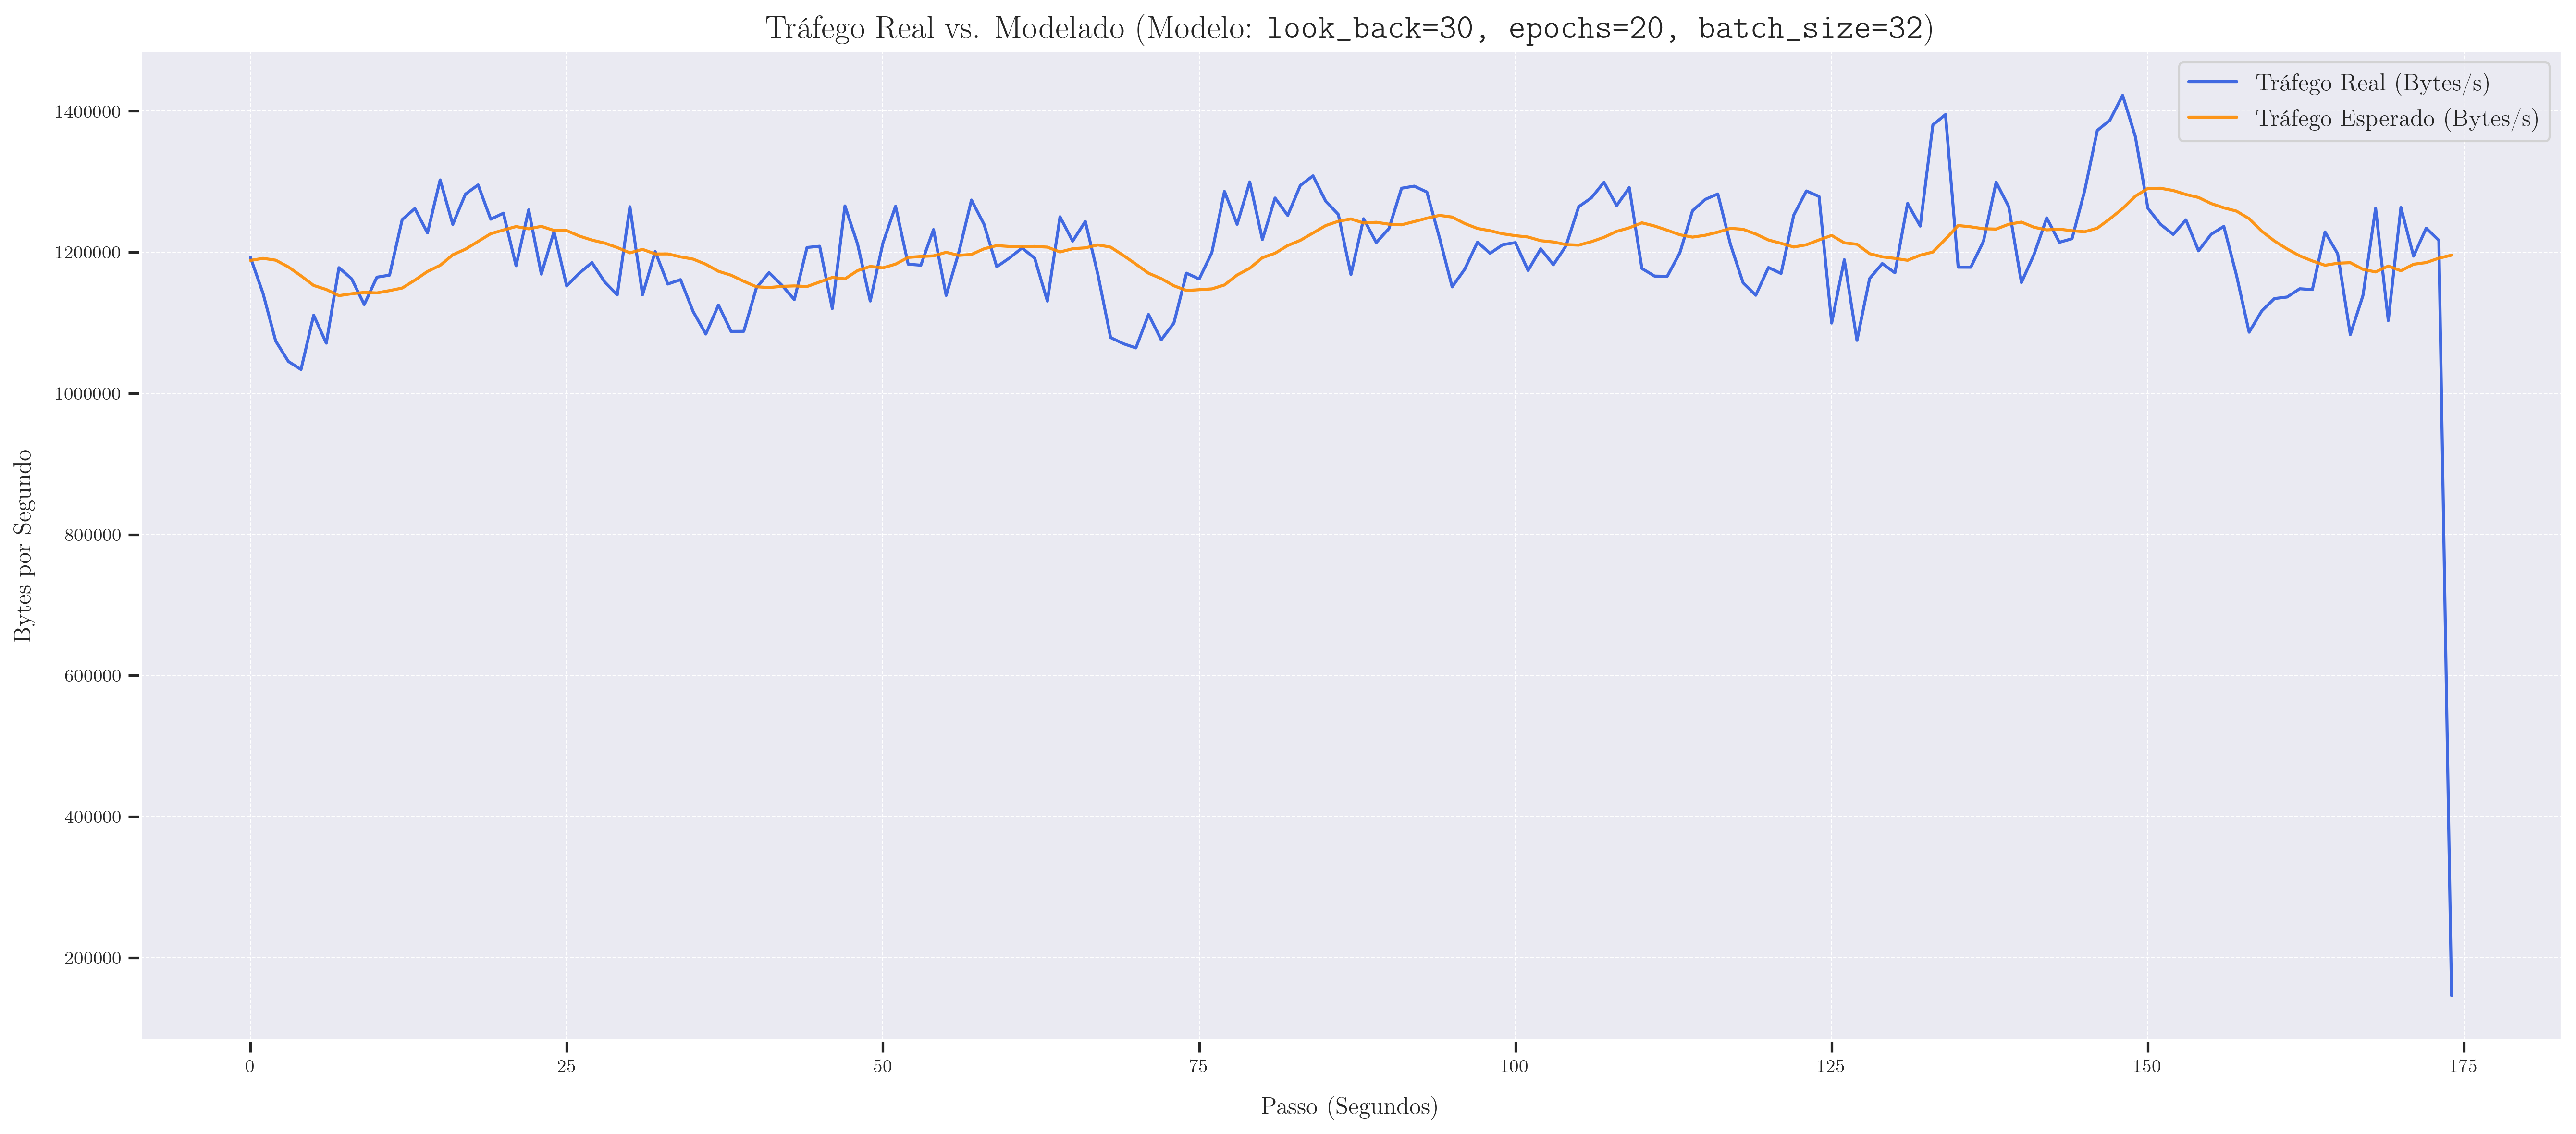
\includegraphics[width=0.95\textwidth]{resource/200701251400.prediction.e20.b32.png}
    \caption{Previsão do modelo com \emph{batch size} de 32 no \emph{dataset} curto.}
    \label{fig:modeling-prediction-reduced}
\end{figure}

Conforme observado na \Cref{tab:modeling-mse-reduced} e na \Cref{fig:modeling-prediction-reduced}, a redução
dos hiperparâmetros de treinamento não resultou em uma diferença significativa na performance ou no
comportamento do modelo em comparação com a execução principal. Isso reforça a conclusão de que a performance
do modelo, neste caso, é mais limitada pela sua arquitetura simples do que pela otimização fina dos
hiperparâmetros de treinamento.
